%%%%%%%%%%%%%%%%%%%%%%%%%%%%%%%%
\section{Memory layout of the unified \ptable-\gtable}
\label{app:seccells:ptable}
%%%%%%%%%%%%%%%%%%%%%%%%%%%%%%%%

\autoref{fig:seccells:ptable_layout} shows the detailed implementation of the
unified \ptable-\gtable in our prototype \seccells implementation.

The table contains a sorted list of cell descriptors, including a
metadata ``cell'' used for storing its sizing parameters.
As described in \autoref{sec:seccells:impl}, each cell descriptor stores virtual 
and physical frame numbers uniquely identifying a VMA, as well as a 
validity flag to track the cell's current validity.
The metadata cell tracks the number of allocated \cell{}s ($N$), the
number of \secdiv{}s ($M$), and sizing factors $T$ (upper bound on \cell count)
and $R$ (upper bound on \secdiv count).
When software requires additional \secdiv{}s or \cell{}s, it must request
the supervisor via a system call.
If the request overflows the bounds imposed by factors $R$ and $T$, the
supervisor must resize this table as required.
The \cell descriptor list is followed by the \ptable, and then by the
\gtable.
This layout assumes, and is optimized, for a cache line size of 64 bytes.

The size of parameters $M$ and $N$, holding the current number of \cell{}s
and \secdiv{}s, in the metadata cell is 32 bits each.
The maximum supported number of \cell{}s in our implementation, therefore,
is $2^{32}$.
The number of \secdiv{}s, however, are limited by the grant table layout.
The 32-bit grant table entries use 29 bits for grantee \secdiv{} identifiers,
thereby limiting the maximum number of \secdiv{}s to $2^{29}$.

\begin{figure*}
  \centering
  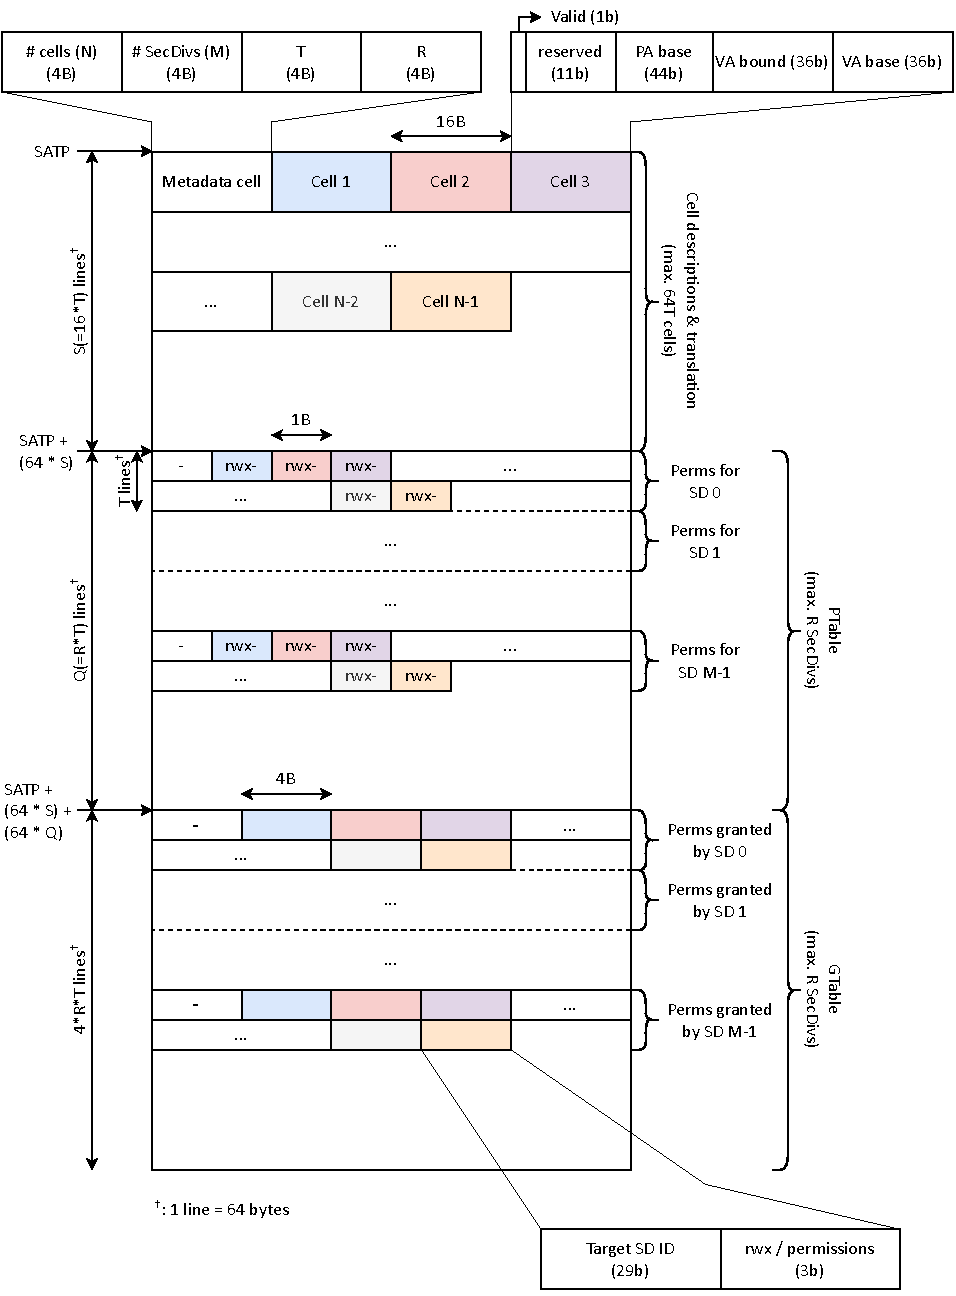
\includegraphics[height=0.95\textheight]{media/seccells/ptable_layout.pdf}
  \caption{Layout of \seccells{}' unified \ptable-\gtable.}
  \label{fig:seccells:ptable_layout}
  %\Description[<short description>]{<long description>}
\end{figure*}

%%%%%%%%%%%%%%%%%%%%%%%%%%%%%%%%
\section{Justification for \autoref{tab:seccells:req_comparison}}
\label{app:seccells:justification_table1}
%%%%%%%%%%%%%%%%%%%%%%%%%%%%%%%%

\paragraph{Obj. \req{1a}}
MPK, ERIM and Donky do not check permissions for instruction fetches, 
simplifying code injection.
Under our threat model, an attacker can inject \Code{wrpkru} instructions 
to corrupt permissions.

\paragraph{Obj. \req{1b}}
Through code injection, call gates in MPK and ERIM can be bypassed.

\paragraph{Obj. \req{1c}}
CODOM requires migrating threads without context isolation.
MPK, ERIM and Donky rely on call gates if context isolation is desired.
However, MPK and ERIM cannot enforce call gates under our threat model.
Donky gives no mechanism for a compartment to restore its state without
trusting general-purpose registers. 
Further, Donky cannot adopt a \seccells-like software approach because a 
compartment has no way to identify itself.

\paragraph{Obj. \req{1d}}
CHERI allows one compartment to unilaterally send a capability to another compartment, 
unchecked by the TCB and unacknowledged by the receiver.

\paragraph{Obj. \req{1e}}
No mechanism except XPC considers the challenge of exclusive access.

\paragraph{Obj. \req{1f}}
A compartment in MPK and ERIM cannot check the value of the \Code{pkru}
register for another compartment, hindering audits.
Cross-core \Code{pkru} reads are not possible.
CHERI requires an expensive full memory scan for capabilities to perform
an audit.

\paragraph{Obj. \req{2a}}
Page-table based translation and permission checking encounter TLB-reach
limits leading to multi-cycle common case access verification for many
widely-used programs including \Code{memcached}. The mechanisms relying on
such page tables for either translation or permission checking fail this
requirement.

\paragraph{Obj. \req{2b}}
Supervisor-mediated cross-compartment calls in UNIX-like OSs,
Mondrian, lwC and CHERI require 100s or 1000s of cycles to complete.

\paragraph{Obj. \req{2c}}
Supervisor-mediated permission transfers are slow (UNIX, MMP, lwC).
MMP proposes the use of redundant mappings with different permissions
to implement a form of zero-copy transfer which is not generic.
CODOM does not really support permission transfers.
XPC restricts permission transfer to a single relay segment.

\paragraph{Obj. \req{3a}}
CODOM identifies the executing compartment by the instruction pointer, 
limiting the flexibility to share code/data regions between compartments.

\paragraph{Obj. \req{3b}}
UNIX, MMP, lwC, XPC and CHERI cannot eliminate context switching when a
permissive policy allows migrating threading between compartments.

%%%%%%%%%%%%%%%%%%%%%%%%%%%%%%%%
\section{Existing mechanisms with \seccells}
\label{app:seccells:integrate_exist}
%%%%%%%%%%%%%%%%%%%%%%%%%%%%%%%%
Many existing performance or security mechanisms can be integrated with
\seccells, either unmodified or with modifications described in this section.

\paragraph{Physical Memory Protections}
\seccells enforces permissions on the virtual address space, and is therefore
trivially compatible with physical memory protection schemes 
including RISC-V's Physical Memory Protection (PMP) mechanism, 
processor reserved memory for Intel's SGX
and vendor-specific protections like Qualcomm's XPU~\cite{qualcomm_ac}.
These mechanisms will apply to the physical address output by 
\seccells' MMU after \ptable access control checks.

\paragraph{Pointer authentication and capabilities}
ARM's pointer authentication code (PAC) feature and CHERI's capabilities
improve memory safety by protecting pointers from illegal 
modifications (overwriting when stored in memory and out-of-bound
increment respectively). Both mechanisms are orthogonal to,
and can integrate with \seccells, which checks accessess against \ptable
permissions when the 
pointers protected by these mechanisms are finally dereferenced, providing
another layer of protection against attacks like PACMAN~\cite{pacmanRavichandranNLY22}.

\paragraph{Hardware and Software Control Flow Integrity}
Hardware (e.g., Intel CET) and software (e.g., LLVM-CFI) control-flow
protections can integrate with \seccells, 
improving intra-compartment control-flow protection to
complement \seccells' inter-compartment call gates (\sdentry).
CET can continue to check indirect call targets for \Code{endbr} instructions. 
LLVM's and other fine-grained CFI pointer checks are implemented in software, 
orthogonal to hardware control flow checks.


\paragraph{Page-based mechanisms}
By itself, \seccells restricts popular mechanisms (e.g., guard pages, swapping)
operating on pages and page tables since translations and protections are 
tracked at \cell granularity.
However, \seccells can be integrated with upcoming intermediate address-space 
systems like Midgard re-enabling programmers to implement these crucial 
features.
Midgard couples \seccells-like range-based translation at the core with
a second level of page-granularity translations at the backside of the 
last-level cache.
Guard pages and swapping can both be implemented by unmapping the requisite pages 
in the backside translation.


%%%%%%%%%%%%%%%%%%%%%%%%%%%%%%%%
\section{\seccells Implementation Trade-Offs}
\label{app:seccells:impl_options}
%%%%%%%%%%%%%%%%%%%%%%%%%%%%%%%%

\seccells permits a range of implementations scaling from simple 
microcontrollers with firmware emulation for added userspace
instructions to server grade processors with microcode or hardware 
implementations. In this section, we describe the trade-offs and 
justify our implementation in \autoref{sec:seccells:impl}.

\paragraph{Firmware}
On the simplest side of the spectrum, instructions can be emulated
by firmware using trap-and-emulate.
Firmware is programmable code which runs in a privileged execution mode 
and uses native ISA instructions.
\seccells' instructions will trap into firmware, and be dispatched to 
the emulation code.
Firmware implementations are cheap, requiring no additional hardware, but 
slower than alternate implementations.
For the simple RISC-V RocketChip microcontroller, we choose 
firmware emulation for permission transfer instructions.
Note that the firmware can also forward traps to be emulated by
either the supervisor or even a privileged userspace library.
However, the additional security risk of emulation by less trusted
software risk and the overhead of forwarding traps makes such
implementations less attractive.

\paragraph{Hardware}
Alternatively, instructions can be implemented in hardware with 
finite-state machine circuits.
While this design option implies better performance,
designing complex hardware comes with silicon and power costs and
substantial complexity.
Hardware bug fixes incur the significant cost of the tape-out process.
Server and desktop processors generally include beefy cores with
large silicon area, where hardware implementations may match the
processor's targeted performance.
We implement the crucial \sdswitch instruction in hardware
to reap the performance advantage,
and because of the simplicity of its design.

\paragraph{Microcode}
A third option, microcode, is programmable code provided by the 
processor manufacturer, built from low level operations including ones 
not available through the ISA interface.
When a instruction implemented in microcode is encountered, a microcode
sequencer fetches microcode from an on-chip RAM and executes them in the
pipeline.
Microcode eliminates the cost of trapping and dispatch encountered in 
firmware emulation ($77\%$ of the latency of emulating \scprot),
and can also leverage hardware-specific optimizations.
Microcode is popular for implementing complicated instructions
with high performance like SGX's \Code{EENTER}/\Code{EEXIT} instructions.
Microcode also has the advantage of being programmable, and have been
leveraged to fix processor errata and bugs.
While the simple RocketChip lacks a microcode sequencer, 
we envision microcode to be ideal for implementing \seccells'
permission transfer instructions for high-performance processors.


%%%%%%%%%%%%%%%%%%%%%%%%%%%%%%%%
\section{\seccells ISA definitions}
\label{app:seccells:isa_def}
%%%%%%%%%%%%%%%%%%%%%%%%%%%%%%%%
Below, we describe the definitions of \seccells' instructions used in our 
RISC-V prototype.

\paragraph{Virtual memory mode} 
\seccells describes an custom virtual memory mode for RISC-V, using the 
\Code{0xf} value for the \Code{Mode} field.

\paragraph{Instruction encodings}
\seccells uses existing spaces left for custom extensions to RISC-V to 
implement the added unprivileged instructions.
Our added instructions occupy the \emph{custom-0} and \emph{custom-1}
spots in RISC-V's instruction encoding map.
\autoref{tab:seccells:instencodings} shows the encoding formats for all
added instructions.

\begin{table}
  \centering
  \begin{tabular}{!l | ?l | ?l | ?l | ?l  }
    \toprule
    \rowstyle\bfseries
    \makecell{\seccells\\instruction} & Arguments              & Output        & \makecell{Prototype\\instruction} & Arguments Mapping                                             \\ \midrule
    SDSwitch                          & addr, SD$_{tgt}$       & return addr   & \Code{JALS}                       & addr = \Code{pc} + \Code{imm}, SD$_{tgt}$ = \Code{rs}         \\
    SDSwitch                          & addr, SD$_{tgt}$       & return addr   & \Code{JALRS}                      & addr = \Code{rs1}, SD$_{tgt}$ = \Code{rs2}                    \\
    SDEntry                           &                        &               & \Code{ENTRY}                      &                                                               \\
    SCProt                            & addr, perm             &               & \Code{PROT}                       & addr = \Code{rs1}, perm = \Code{rs2}                          \\
    SCGrant                           & addr, SD$_{tgt}$, perm &               & \Code{GRANT}                      & addr = \Code{rs1}, SD$_{tgt}$ = \Code{rs2}, perm = \Code{imm} \\
    SCRecv                            & addr, SD$_{src}$, perm &               & \Code{RECV}                       & addr = \Code{rs1}, SD$_{src}$ = \Code{rs2}, perm = \Code{imm} \\
    SCTfer                            & addr, SD$_{tgt}$, perm &               & \Code{TFER}                       & addr = \Code{rs1}, SD$_{tgt}$ = \Code{rs2}, perm = \Code{imm} \\
    SCReval                           & addr, perm             &               & \Code{REVAL}                      & addr = \Code{rs1}, perm = \Code{rs2}                          \\
    SCInval                           & addr                   &               & \Code{INVAL}                      & addr = \Code{rs1}                                             \\
    SCExcl                            & addr, perm             & True/False    & \Code{EXCL}                       & addr = \Code{rs1}, perm = \Code{rs2}                          \\ \bottomrule
  \end{tabular}
  \label{tab:seccells:instmapping}
  \caption[Mapping \seccells instructions to the RISC-V prototype instructions]
          {Mapping \seccells instructions and arguments to the RISC-V prototype instructions. 
          Instructions returning values write to the \Code{rd} register}
\end{table}

\begin{table}
  \centering
  \begin{tabular}{| !c | ?c | ?c | ?c | ?c | ?c | ?l |}
    \toprule
    \multicolumn{6}{|c|}{\textbf{Instruction Fields}}                                                                  & \textbf{Type}                \\ \midrule
    \Code{func7}         & \Code{rs2    }     & \Code{rs1}       & \Code{func3}    & \Code{rd}       & \Code{opcode}   & R-type                       \\ \hline    
    \multicolumn{2}{|c|}{\Code{imm[11:0]}}    & \Code{rs1}       & \Code{func3}    & \Code{rd}       & \Code{opcode}   & I-type                       \\ \hline    
    \Code{imm[11:5]}     & \Code{rs2    }     & \Code{rs1}       & \Code{func3}    & \Code{imm[4:0]} & \Code{opcode}   & S-type                       \\ \hline
    \multicolumn{4}{|c|}{\Code{imm[20|10:1|11|19:12]}}                             & \Code{rd}       & \Code{opcode}   & J-type                       \\ \bottomrule    
    \multicolumn{7}{c}{ }                                                                                                                             \\ \toprule
    \multicolumn{6}{|c|}{\textbf{Encodings}}                                                                           & \textbf{Instruction}         \\ \midrule
    \multicolumn{4}{|c|}{\Code{imm[20:1]}}                                         & \Code{rs/rd   } & \Code{0101011}  & \Code{JALS(rs, imm) = rd  }  \\ \hline   
    \Code{0000000  }     & \Code{rs2    }     & \Code{rs1    }   & \Code{000}      & \Code{rd      } & \Code{0001011}  & \Code{JALRS(rs1, rs2) = rd}  \\ \hline  
    \multicolumn{2}{|c|}{\Code{000000000000}} & \Code{rs1 = 0}   & \Code{001}      & \Code{rd = 0  } & \Code{0001011}  & \Code{ENTRY               }  \\ \hline  
    \Code{1000000  }     & \Code{rs2 = 0}     & \Code{rs1    }   & \Code{010}      & \Code{rd = 0  } & \Code{0001011}  & \Code{INVAL(rs1)          }  \\ \hline    
    \Code{0000000  }     & \Code{rs2    }     & \Code{rs1    }   & \Code{010}      & \Code{rd = 0  } & \Code{0001011}  & \Code{REVAL(rs1, rs2)     }  \\ \hline  
    \Code{0000000  }     & \Code{rs2    }     & \Code{rs1    }   & \Code{011}      & \Code{rd = 0  } & \Code{0001011}  & \Code{PROT(rs1, rs2)      }  \\ \hline     
    \Code{imm[11:5]}     & \Code{rs2    }     & \Code{rs1    }   & \Code{100}      & \Code{imm[4:0]} & \Code{0001011}  & \Code{GRANT(rs1, rs2, imm)}  \\ \hline   
    \Code{imm[11:5]}     & \Code{rs2    }     & \Code{rs1    }   & \Code{101}      & \Code{imm[4:0]} & \Code{0001011}  & \Code{TFER(rs1, rs2, imm) }  \\ \hline   
    \Code{imm[11:5]}     & \Code{rs2    }     & \Code{rs1    }   & \Code{110}      & \Code{imm[4:0]} & \Code{0001011}  & \Code{RECV(rs1, rs2, imm) }  \\ \hline   
    \Code{0000000  }     & \Code{rs2    }     & \Code{rs1    }   & \Code{111}      & \Code{rd      } & \Code{0001011}  & \Code{EXCL(rs1, rs2) = rd }  \\ \bottomrule
  \end{tabular}
  \label{tab:seccells:instencodings}
  \caption[Instruction encodings for \seccells' prototype]
          {Instruction encodings for \seccells' prototype. 
          The first part shows the four instruction encoding types supported by RISC-V.}
\end{table}

\paragraph{Exception details}
\seccells also adds new exceptions, corresponding to failed security checks
while executing the added unprivileged instructions.
\autoref{tab:seccells:exceptions} lists the added exceptions, and the 
corresponding values for the \Code{scause} and \Code{stval} registers
storing exception details.

\begin{table}[t]
  \centering
  \begin{tabular}{ !l | ?l | ?l | ?l }
    \toprule
    \rowstyle\bfseries
    Instruction & Exception Cause             & \Code{scause} code                & \Code{stval}                                                                            \\ \midrule
    EXCL        & Illegal address             & \Code{\_ILL\_ADDR}                & addr                                                                                    \\ \hline
    EXCL        & Illegal permissions         & \Code{\_ILL\_PERM}                & \makecell[l]{
                                                                                      (type $\ll$ 8) | perm                                                                 \\
                                                                                      type = 
                                                                                      $
                                                                                        \begin{cases}
                                                                                          \text{0} &\text{if perm not in RWX}                                               \\
                                                                                          \text{1} &\text{if perm is zero}                                                  \\
                                                                                          \text{2} &\text{\makecell[l]{if SD$_{cur}$ has insufficient \\perms}}             \\
                                                                                        \end{cases}
                                                                                      $
                                                                                    }                                                                                       \\ \hline
    EXCL        & Cell description invalid    & \Code{\_INV\_CELL\_STATE}         & 0 if cell is invalid                                                                    \\ \hline
    GRANT       & Illegal address             & \Code{\_ILL\_ADDR}                & addr                                                                                    \\ \hline
    GRANT       & Target too high             & \Code{\_INV\_SDID}                & SD$_{tgt}$                                                                              \\ \hline
    GRANT       & Illegal permissions         & \Code{\_ILL\_PERM}                & \makecell[l]{                                              
                                                                                      (type $\ll$ 8) | perm                                                                 \\
                                                                                      type = 
                                                                                      $
                                                                                        \begin{cases}
                                                                                          \text{0} &\text{if perm not in RWX}                                               \\
                                                                                          \text{1} &\text{if perm is zero}                                                  \\
                                                                                          \text{2} &\text{\makecell[l]{if SD$_{cur}$ has insufficient \\perms}}             \\
                                                                                        \end{cases}
                                                                                      $
                                                                                    }                                                                                       \\ \hline
    GRANT       & Cell description invalid    & \Code{\_INV\_CELL\_STATE}         & 0 if cell is invalid                                                                    \\ \hline
    RECV        & Illegal address             & \Code{\_ILL\_ADDR}                & addr                                                                                    \\ \hline
    RECV        & Cell description invalid    & \Code{\_INV\_CELL\_STATE}         & 0 if cell is invalid                                                                    \\ \hline
    RECV        & Illegal permissions         & \Code{\_ILL\_PERM}                & \makecell[l]{                                              
                                                                                      (type $\ll$ 8) | perm                                                                 \\
                                                                                      type = 
                                                                                      $
                                                                                        \begin{cases}
                                                                                          \text{0} &\text{if perm not in RWX}                                               \\
                                                                                          \text{1} &\text{if perm is zero}                                                  \\
                                                                                          \text{3} &\text{\makecell[l]{if requested perms not \\subset of granted perms}}   \\
                                                                                        \end{cases}
                                                                                      $
                                                                                    }                                                                                       \\ \hline
    RECV        & Invalid SD                  & \Code{\_INV\_SDID}                & \makecell[l]{
                                                                                      (type $\ll$ 32) | SD                                                                  \\
                                                                                      type =
                                                                                      $
                                                                                        \begin{cases}
                                                                                          \text{0} &\text{\makecell[l]{if SD source too high\\ or SD=SD$_{src}$}}                           \\
                                                                                          \text{1} &\text{\makecell[l]{if grant SD != SD$_{cur}$\\ or SD=SD$_{cur}$}}                       \\
                                                                                        \end{cases}
                                                                                      $
                                                                                    }                                                                                       \\ \hline
    PROT        & Illegal address             & \Code{\_ILL\_ADDR}                & addr                                                                                    \\ \hline
    PROT        & Illegal permissions         & \Code{\_ILL\_PERM}                & \makecell[l]{                                              
                                                                                      (type $\ll$ 8) | perm                                                                 \\
                                                                                      type = 
                                                                                      $
                                                                                        \begin{cases}
                                                                                          \text{0} &\text{if perm not in RWX}                                               \\
                                                                                          \text{2} &\text{\makecell[l]{if SD$_{cur}$ has insufficient \\perms}}             \\
                                                                                        \end{cases}
                                                                                      $
                                                                                    }                                                                                       \\ \hline
    PROT        & Cell description invalid    & \Code{\_INV\_CELL\_STATE}         & 0 if cell is invalid                                                                    \\ \hline
    TFER        & Illegal address             & \Code{\_ILL\_ADDR}                & addr                                                                                    \\ \hline
    TFER        & Target too high             & \Code{\_INV\_SDID}                & SD$_{tgt}$                                                                              \\ \hline
    TFER        & Illegal permissions         & \Code{\_ILL\_PERM}                & \makecell[l]{                                              
                                                                                      (type $\ll$ 8) | perm                                                                 \\
                                                                                      type = 
                                                                                      $
                                                                                        \begin{cases}
                                                                                          \text{0} &\text{if perm not in RWX}                                               \\
                                                                                          \text{1} &\text{if perm is zero}                                                  \\
                                                                                          \text{2} &\text{\makecell[l]{if SD$_{cur}$ has insufficient \\perms}}             \\
                                                                                        \end{cases}
                                                                                      $
    }                                                                                       \\ \bottomrule
  \end{tabular}
  \caption[\seccells exception codes]
          {Exception causes, \Code{scause} and \Code{stval} register values for \seccells exceptions}
  \label{tab:seccells:exceptions}
\end{table}

\begin{table}[t]
  \ContinuedFloat
  \begin{tabular}{ !l | ?l | ?l | ?l }
    \toprule
    \rowstyle\bfseries
    Instruction & Exception Cause             & \Code{scause} code                & \Code{stval}                                                                            \\ \midrule
    TFER        & Cell description invalid    & \Code{\_INV\_CELL\_STATE}         & 0 if cell is invalid                                                                    \\ \hline
    INVAL       & Illegal address             & \Code{\_ILL\_ADDR}                & addr                                                                                    \\ \hline
    INVAL       & Cell description invalid    & \Code{\_INV\_CELL\_STATE}         & \makecell[l]{
                                                                                      type                                                                                  \\
                                                                                      type = 
                                                                                      $
                                                                                        \begin{cases}
                                                                                          \text{0} &\text{if cell is already invalid}                                       \\
                                                                                          \text{2} &\text{if other SD has non-zero perms}                                   \\
                                                                                          \text{3} &\text{outstanding grants for cell}                                      \\
                                                                                        \end{cases}
                                                                                      $
                                                                                    }                                                                                       \\ \hline
    REVAL       & Illegal address             & \Code{\_ILL\_ADDR}                & addr                                                                                    \\ \hline
    REVAL       & Cell description invalid    & \Code{\_INV\_CELL\_STATE}         & 1 if cell is already valid                                                              \\ \hline
    REVAL       & Illegal permissions         & \Code{\_ILL\_PERM}                & \makecell[l]{                                              
                                                                                      (type $\ll$ 8) | perm                                                                 \\
                                                                                      type = 
                                                                                      $
                                                                                        \begin{cases}
                                                                                          \text{0} &\text{if perm not in RWX}                                               \\
                                                                                          \text{1} &\text{if perm is zero}                                                  \\
                                                                                        \end{cases}
                                                                                      $
                                                                                    }                                                                                       \\ \hline
    JAL(R)S     & Target too high             & \Code{\_INV\_SDID}                & SD$_{tgt}$                                                                              \\ \hline
    JAL(R)S     & Illegal target instruction  & \Code{\_ILL\_TGT}                 & Target addr                                                                             \\ \bottomrule
  \end{tabular}
  \caption[]
          {(cont.) Exception causes, \Code{scause} code and \Code{stval} register values for \seccells exceptions}
  \label{tab:seccells:exceptions}
\end{table}

\begin{table}
  \centering
  \begin{tabular}{ !l | ?l }
    \toprule
    \rowstyle\bfseries
    \Code{scause} code        & Value  \\ \midrule
    \Code{\_ILL\_ADDR}        & 0x18   \\
    \Code{\_ILL\_PERM}        & 0x19   \\
    \Code{\_INV\_SDID}        & 0x1a   \\
    \Code{\_INV\_CELL\_STATE} & 0x1b   \\
    \Code{\_ILL\_TGT}         & 0x1c   \\ \bottomrule

  \end{tabular}
  \caption{Mapping \seccells exception codes to values}
  \label{tab:seccells:exceptioncodes}
\end{table}

%%%%%%%%%%%%%%%%%%%%%%%%%%%%%%%%
\section{Accelerating \seccells Instruction Emulation}
\label{app:seccells:trapacceleration}
%%%%%%%%%%%%%%%%%%%%%%%%%%%%%%%%

%-------------------------------
\subsection{Generic Trap-and-Emulate Acceleration}
%-------------------------------
The RISC-V architecture embraces the trap-and-emulate mechanism for
maintaining software compatibility across a wide range of hardware.
Essentially, beefier cores can implement complex instructions in hardware
where leaner cores can rely on traps into the firmware which emulates
the same instructions in software.
\seccells' prototype utilizes the trap-and-emulate mechanism for
implementing permission modification and transfer instructions 
(\scprot, \scgrant, \screcv, \sctfer, \screval, \scinval, \scexcl),
in line with the complexity of the RocketChip core which resembles
an embedded processor.
To accelerate the instruction emulation, our prototype also introduces a 
mechanism for accelerating the trap-and-emulate mechanism.
The mechanism described below is generic, and not
restricted to emulating \seccells' instructions.

The naive trap-and-emulate mechanism relies on saving the
core's entire general-purpose register (GPR) context to memory, 
to later read argument registers for the emulated instruction.
Consequently, the trap-and-emulate mechanism is relatively costly,
consuming almost a hundred cycles to just switch contexts.
Since the firmware can only find the argument register after reading the
trapping instruction, decoding the instruction in software and finding
the argument register fields, saving every register is essential.

While illegal instruction traps can originate from actually illegal
byte sequences in code, the trap-and-emulate mechanism applies to
actually valid instruction encodings.
These instructions are fetched, and pass through the decode stage, which
deciphers the instruction's encoding and the argument register names
before raising the illegal instruction trap.
We realized that the hardware can, therefore, read and save the relevant
argument registers to special system registers allowing the firmware to
directly access register arguments.
Moreover, traps cause a pipeline flush, allowing the decode stage to ensure
that the most recent value of the architectural register is saved to
the special registers, even in an out-of-order core.
The firmware, therefore, can include fast paths for trap-and-emulate,
only storing the registers overwritten by the firmware during emulation to
save tens of cycles.
The firmware also saves cycles used for entirely decoding instructions to
find their argument registers.
For instructions which can be emulated in tens or a hundred cycles,
including the aforementioned \seccells instructions, saving tens of cycles
during trap entry and exit can account for a significant speedup of
up to $70\%$.

Our FPGA prototype, therefore, implements five extra machine-mode 
control-and-status registers (CSRs)
for handling instruction arguments for trapping instructions.
Three read-only registers, \Code{mtirs1}, \Code{mtirs2} and \Code{mtiimm}
store the argument register values, and the immediate value as relevant to 
the trapping instruction.
These registers can directly be read by the firmware during emulation.
A fourth read-only register, \Code{mtird} stores the name of the
destination register, if required by the trapped instruction.
A write-only register, \Code{mtirdval} can be written to by the firmware
during instruction emulation, representing the value generated by the
instruction.
When the trap returns, the \Code{mret} instruction writes the returned value
into the correct destination register.
Instructions without an output will have the \Code{mtird} register pointing
to the \Code{x0} register, which is hardware pinned to the value zero.


%-------------------------------
\subsection{\seccells-specific \ptable-\gtable Access Helpers}
%-------------------------------
\seccells' PTable structure is designed to specifically make lookups for
\cell descriptions and permissions straightforward.
The addresses of permissions and descriptions can be generated with
simple arithmetic involving addition and bit-shift operations.
Our prototype exposes single instructions for generating addresses
within the \ptable and for checking permissions in the \ptable, 
implemented as simple hardware arithmetic circuits.
The four instructions are listed below.
\begin{itemize}
  \item \textbf{Check cell} The \Code{SCCCK} instruction resembles ARM's
    \Code{AT} instruction~\cite{ARMAT}, and allows the firmware to check
    whether a instruction has a valid translation by accessing the core's
    range-TLB.

  \item \textbf{Cell Address} Generates the address for the cell description for
    a cell with a specified index.

  \item \textbf{Permission Address} Generates the address for the permissions
    byte within the \ptable for a specific \cell and \secdiv.

  \item \textbf{Grant Address} Generates the address for the grant table entry
    within the \gtable for a specific \cell and \secdiv.
\end{itemize}


